\aufgabenblatt{1}

\ifcomment\else
\subsection*{Zweck, Ablauf und Studienleistung}

Die Praktische Übung (PÜ) zur \href{https://ekvv.uni-bielefeld.de/kvv_publ/publ/vd?id=389104149}{Vorlesung Zeitreihenanalyse} unterstützt Sie bei der Festigung des Lernstoffes durch eigenständige Auseinandersetzung mit Problemen. Wir werden auch den Umgang mit \texttt{R} trainieren. Die Teilnahme ist keine Klausurvoraussetzung. Unsere Treffen finden 14-tägig am Montag von 16:15 bis 17:45 Uhr statt, die \href{https://ekvv.uni-bielefeld.de/kvv_publ/publ/Veranstaltung_Termine.jsp?id=388066971}{Einzeltermine stehen im eKVV}. Die Treffen sind zweigeteilt: Im ersten Teil bearbeiten Sie selbstständig Aufgaben und haben die Möglichkeit, mir persönlich Fragen zu stellen. Im zweiten Teil werden die Aufgaben im Plenum besprochen. Alle Aufgabenblätter und Lösungen finden Sie im \href{https://moodle.uni-bielefeld.de/course/view.php?id=1035}{Lernraum der PÜ}. \\

Sie können eine Studienleistung für die Module \href{https://ekvv.uni-bielefeld.de/sinfo/publ/modul/26802869}{31-M23} oder \href{https://ekvv.uni-bielefeld.de/sinfo/publ/modul/47135019}{31-SW-StaM} erwerben. Dafür müssen Sie zwei Leistungen erbringen:
\begin{itemize}
    \item \textbf{Präsentation einer Aufgabe:} Sie präsentieren einmalig Ihre Lösungsansätze für eine selbstgewählte Aufgabe. Im \href{https://moodle.uni-bielefeld.de/course/view.php?id=1035}{Lernraum der PÜ} können Sie sich eine Aufgabe reservieren.
    \item \textbf{Analyse einer Zeitreihe:} Sie analysieren eine selbstgewählte Zeitreihe mit den in der Vorlesung präsentierten Verfahren und erstellen einen Kurzbericht.
    \begin{itemize}
        \item \textbf{Anforderungen an die Zeitreihe:} Mindestens intervallskaliert; zwischen 100 und 1000 Beobachtungen; Tages-, Wochen-, Monats- oder Quartalsdaten; Trend und Saisonalität sollen erkennbar sein (saisonbereinigte Daten und Finanzzeitreihen im Allgemeinen sind ungeeignet); Beispiele für Datenquellen: \href{https://www-genesis.destatis.de/genesis/online}{Statistisches Bundesamt}, \href{https://ec.europa.eu/eurostat/de/}{Statistisches Amt der Europäischen Union}, \href{https://www.kaggle.com/datasets?search=time+series}{Kaggle} (siehe Abbildung \ref{fig:zeitreihe_beispiele}).
        \item \textbf{Anforderungen an die Analyse:} Inhaltliche Beschreibung der Zeitreihe; Quellenangabe; grafische Darstellungen; Zerlegung mit dem Komponentenmodell; Prognose über die zukünftige Entwicklung; Analysebericht mit \texttt{R Markdown} (siehe Aufgabe 2).
        \item \textbf{Abgabe:} 
        Bitte ausschließlich über den \href{https://moodle.uni-bielefeld.de/course/view.php?id=1035}{Lernraum der PÜ}, nicht per E-Mail.
        \begin{itemize}
            \item[1.] Bis zum \textbf{30. April} laden Sie Ihre Zeitreihe im \texttt{.csv}-Format hoch. Im Kommentarbereich geben Sie bitte die Datenquelle sowie eine kurze Rechtfertigung an, warum Ihre Zeitreihe den obigen Anforderungen entspricht.
            \item[2.] Bis zum \textbf{30. Juni} laden Sie Ihren Bericht im \texttt{.Rmd}- und \texttt{.pdf}-Format hoch.
        \end{itemize}
    \end{itemize}
\end{itemize}
\enlargethispage{3cm}
\vspace{-0.5cm}
\begin{figure}[!h]
    \centering
    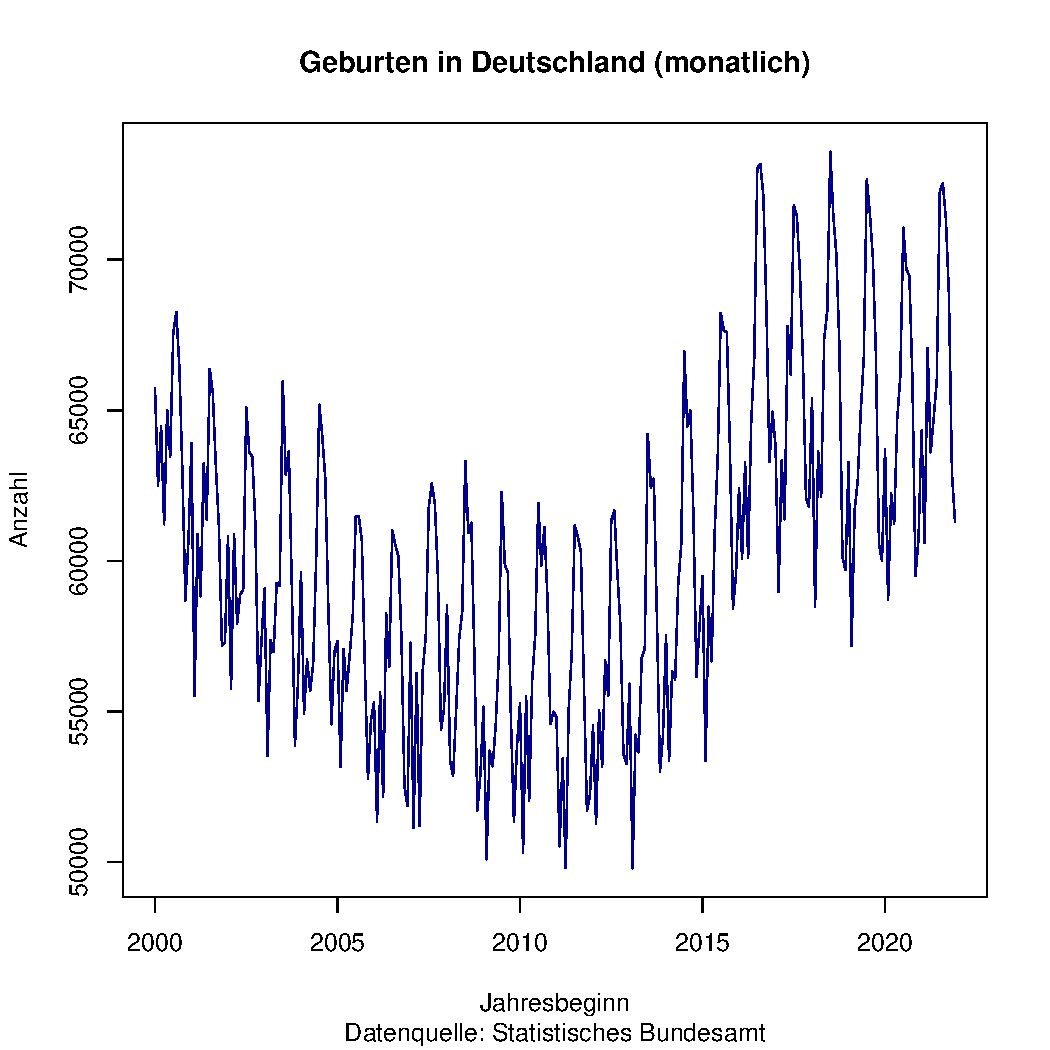
\includegraphics[width = .3\textwidth]{resources/geburten.pdf}
    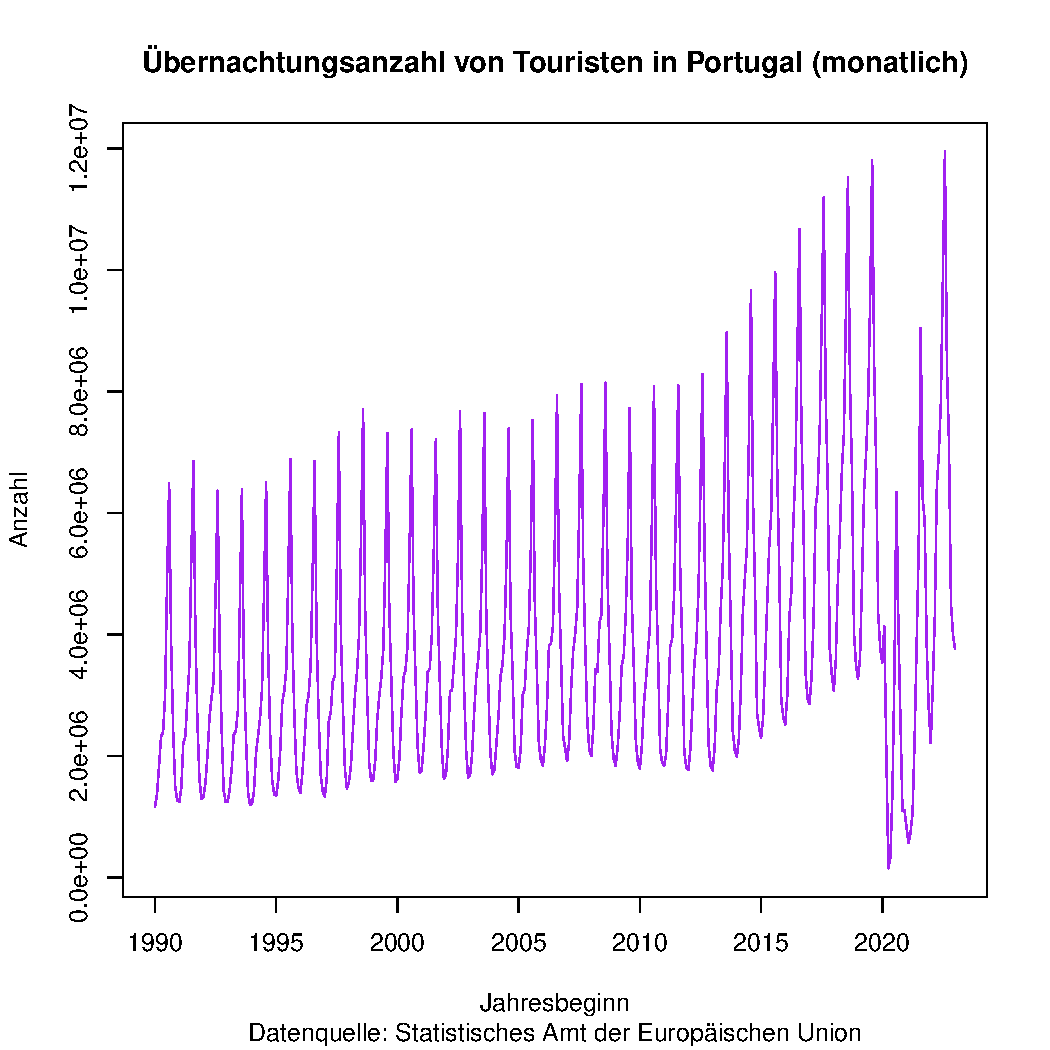
\includegraphics[width = .3\textwidth]{resources/uebernachtungen.pdf}
    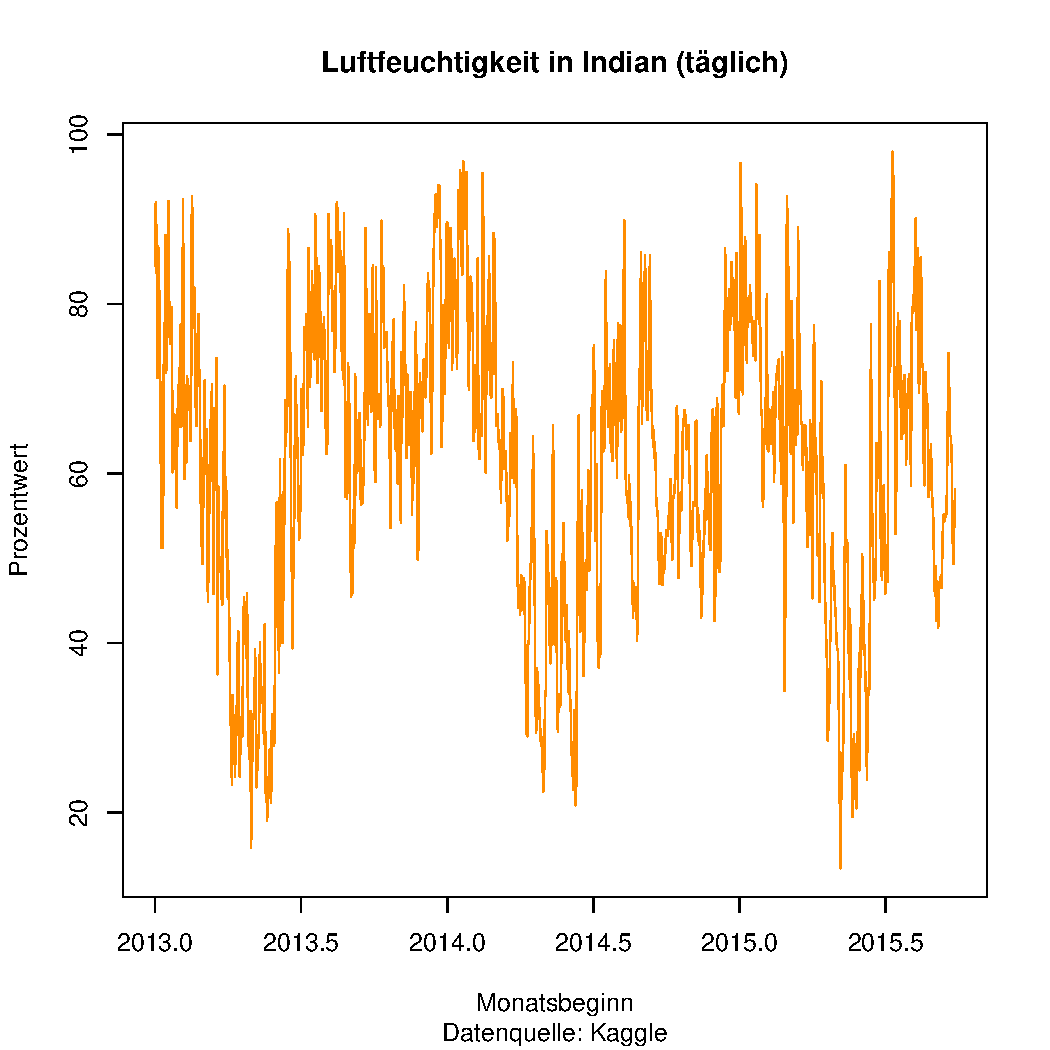
\includegraphics[width = .3\textwidth]{resources/luftfeuchtigkeit.pdf}
    \caption{Drei Beispiele für geeignete Zeitreihen. Im \href{https://moodle.uni-bielefeld.de/course/view.php?id=1035}{Lernraum der PÜ} finden Sie den \texttt{R} Code, mit dem die Zeitreihen downgeloadet und visualisiert wurden.}
    \label{fig:zeitreihe_beispiele}
\end{figure}
\fi

\aufgabe{1}{Einführung in \texttt{R}}

\begin{enumerate}

\item Die Dokumentation \emph{simpleR} von John Verzani liefert eine gute Einführung in \texttt{R}. Downloaden Sie das Dokument via \href{http://cran.r-project.org/doc/contrib/Verzani-SimpleR.pdf}{http://cran.r-project.org/doc/contrib/Verzani-SimpleR.pdf} und lesen Sie \emph{Section 2: Data}, um zu lernen, wie Datensätze mit der \texttt{c()} Funktion eingegeben werden können. Erzeugen Sie anschließend folgende zwei Vektoren in \texttt{R}:
\setcounter{MaxMatrixCols}{11}
\begin{align*}
x^\top &=
\begin{bmatrix}
10 & 8 & 13 & 9 & 11 & 14 & 6 & 4 & 12 & 7 & 5
\end{bmatrix}
\\
y^\top &=
\begin{bmatrix}
8.1 & 6.9 & 7.5 & 8.8 & 8.3 & 9.9 & 7.2 & 4.2 & 10.8 & 4.8 & 5.6
\end{bmatrix}
\end{align*}

\comment{
\texttt{x <- c(10, 8, 13, 9, 11, 14, 6, 4, 12, 7, 5) \\
y <- c(8.1, 6.9, 7.5, 8.8, 8.3, 9.9, 7.2, 4.2, 10.8, 4.8, 5.6)}
}

\item Welche Operation wird durch \texttt{x + y} ausgeführt? Wenden Sie auch \texttt{-, *, /, \%*\%} an.

\comment{
\texttt{x + y} ist die elementweise Addition. Analog sind \texttt{-, *, /} die elementweise Subtraktion, Multiplikation und Division. \texttt{x \%*\% y} ist das Matrikprodukt $x^\top y$.
}

\item Die Einträge der beiden Vektoren können wir als Wertepaare $(x_1,y_1), \ldots, (x_{11}, y_{11})$ betrachten. Erzeugen Sie mit \texttt{plot()} ein Streudiagramm dieser Daten.

\comment{
\texttt{plot(x, y)}
}

\item Lesen Sie \emph{Section 5: Multivariate Data} und lernen Sie den Datentyp \texttt{data.frame} kennen. Erstellen Sie einen \texttt{data.frame} aus \texttt{x} und \texttt{y}.

\comment{
\texttt{data <- data.frame(x = x, y = y)}
}

\item Schätzen Sie die Koeffizienten $\beta_0$ und $\beta_1$ des linearen Modells $y = \beta_0 + \beta_1 x + u$ mithilfe der Funktion \texttt{lm()} (steht für \emph{lineares Modell}). Erklärungen finden Sie in \emph{Section 13: Regression Analysis}. Zeichnen Sie dann mithilfe von \texttt{abline()} die angepasste Regressionsgerade in Ihr Streudiagramm ein.

\comment{
\texttt{model <- lm(formula = y \~{} x, data = data) \\
abline(model)
}
}

\item Erklären Sie den Output von \texttt{summary()}, angewendet auf Ihr geschätztes Modell.

\comment{
\texttt{summary(model)} \\
Eine Erklärung des Outputs liefert \href{https://www.youtube.com/watch?v=NEfjirpOj7s}{https://www.youtube.com/watch?v=NEfjirpOj7s}.}

\end{enumerate}

\aufgabe{2}{Einführung in \texttt{R Markdown}}

\texttt{R Markdown} ist eine Kombination aus \texttt{R}, unserer Programmiersprache für Datenanalyse, und \texttt{Markdown}, einer einfachen Auszeichnungssprache für die Erstellung von Berichten. Durch die Kombination können wir \texttt{R} Code direkt in Textdokumente integrieren und mit minimalem Aufwand dynamische Analyseberichte generieren. Entwickelt wurde \texttt{R Markdown} 2014 von Yihui Xie, der einen \href{https://www.youtube.com/watch?v=LussVnrLZKU}{einfachen Weg gesucht hat, seine \texttt{R} Hausaufgaben aufzuschreiben}.

\begin{enumerate}

\item Das Buch \emph{R for Data Science} von Hadley Wickham bietet unter anderem eine gute Einführung in \texttt{R Markdown}. Das Buch ist kostenlos online unter \href{https://r4ds.had.co.nz/}{https://r4ds.had.co.nz/} verfügbar. Lesen Sie \emph{Chapter 27: R Markdown}, um zu lernen, wie ein \texttt{R Markdown} Dokument erstellt werden kann. Verwenden Sie die Vorlage aus Abschnitt 27.2 und erstellen Sie selbst ein \texttt{R Markdown} Dokument im \texttt{.html}-Format.

\comment{Dazu in R Studio links oben \texttt{File > New File > R Markdown} wählen. Es öffnet sich ein Fenster, dort links unten auf \texttt{Create Empty Document} klicken. Es öffnet sich eine leere Datei, dort die Vorlage einfügen. Anschließend auf \texttt{Knit} klicken.}
    
\item Fügen Sie in das \texttt{R Markdown} Dokument Ihre Lösungen aus Aufgabe 1) ein.

\ifcomment
\begin{framed}
\begin{minipage}[fragile]{0.9\textwidth}
\begin{verbatim}
---
title: "Lösung zu Aufgabe 1"
date: "17.04.2023"
author: "Lennart"
output: html_document
---
### a)
```{r}
x <- c(10, 8, 13, 9, 11, 14, 6, 4, 12, 7, 5)
y <- c(8.1, 6.9, 7.5, 8.8, 8.3, 9.9, 7.2, 4.2, 10.8, 4.8, 5.6)
```
\end{verbatim}
\end{minipage}
\end{framed}
\fi

\item Wie können Sie ein \texttt{.pdf}-Dokument erstellen?
\comment{Indem \texttt{output: html\_document} durch \texttt{output: pdf\_document} ersetzt wird.}

\end{enumerate}



